\section{Alternatives to Naive Bayes}
As a classifier is modelled after some given assumptions and with specific architectural proprieties, e.g. all attributes are equally important, it is important to check if the used classifier is the right model for the examined problem.
A very good feature of the Naive Bayes classifier is its ability to train on a dataset with a very high dimensionality in decent time.
Because this property is not shared among all other classifier and some even severely suffer from high dimensionality (the so called Curse of Dimensionality \cite{bellman1957dynamic}), we are using the reduced set of features we estimated in the feature selection process without further research on the impact of other thresholds on feature trimming w.r.t. to non-bayesian classifiers.

\subsection{Decision Trees}

We are going to use Weka's \cite{hall2009weka} implementation of the C4.5 decision tree \cite{Quinlan1993} (known in Weka as J48) as the first alternative to Naive Bayes classification.
C4.5 builds a tree based on the features using information entropy.
The dimension with the highest information gain will be used at each node to generate a new split.
After the creation of the tree, C4.5 tries to prune all unnecessary branches into simple leafs to keep the total number of nodes to a minimum.
Although this feature could be disabled, we are using it to avoid overfitting.

As the runtime of C4.5 increases in a higher level with the number of dimensions than the Naive Bayes classifier, we are going to use it with the thresholds $\alpha=0.017$ and $\beta=0.19$.
This reduced data set of only 1568 dimensions can be used to train a C4.5 tree in a feasible amount of time.

\begin{figure}[h!]
    \centering
    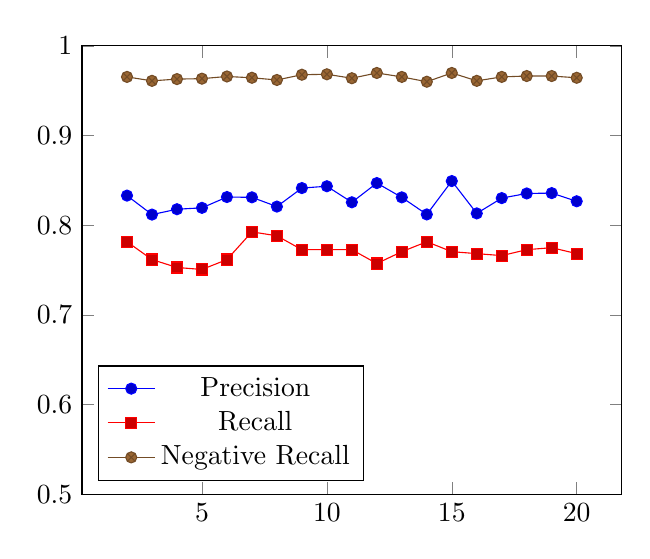
\begin{tikzpicture}
        \begin{axis}[
            legend pos=south west,
            ymax=1,
            ymin=0.5
            ]
            \addplot+[sharp plot] coordinates {
            (2, 0.832941)
            (3, 0.811765)
            (4, 0.817746)
            (5, 0.819277)
            (6, 0.831325)
            (7, 0.831019)
            (8, 0.820690)
            (9, 0.841346)
            (10, 0.843373)
            (11, 0.825472)
            (12, 0.846914)
            (13, 0.830952)
            (14, 0.811927)
            (15, 0.849148)
            (16, 0.813084)
            (17, 0.830144)
            (18, 0.835322)
            (19, 0.835714)
            (20, 0.826603)
            };
            \addlegendentry{Precision}
            \addplot+[sharp plot] coordinates {
            (2, 0.781457)
            (3, 0.761589)
            (4, 0.752759)
            (5, 0.750552)
            (6, 0.761589)
            (7, 0.792494)
            (8, 0.788079)
            (9, 0.772627)
            (10, 0.772627)
            (11, 0.772627)
            (12, 0.757174)
            (13, 0.770419)
            (14, 0.781457)
            (15, 0.770419)
            (16, 0.768212)
            (17, 0.766004)
            (18, 0.772627)
            (19, 0.774834)
            (20, 0.768212)
            };
            \addlegendentry{Recall}
            \addplot+[sharp plot] coordinates {
            (2, 0.965315)
            (3, 0.960918)
            (4, 0.962872)
            (5, 0.963361)
            (6, 0.965804)
            (7, 0.964338)
            (8, 0.961895)
            (9, 0.967758)
            (10, 0.968246)
            (11, 0.963850)
            (12, 0.969712)
            (13, 0.965315)
            (14, 0.959941)
            (15, 0.969712)
            (16, 0.960918)
            (17, 0.965315)
            (18, 0.966292)
            (19, 0.966292)
            (20, 0.964338)
            };
            \addlegendentry{Negative Recall}
        \end{axis}
    \end{tikzpicture}
    \caption{Performance of J48 w.r.t. the number of minimum instances per leaf}
    \label{fig:j48}
\end{figure}



One of the parameters that can be adjusted is the number of instances each leaf of the tree needs to represent at least during the training phase.
The default setting of WEKA requires at minimum two instances at each leaf, in Figure \ref{fig:j48} we outline the scores with varying number of minimum instances.
From the results we can see that changing the minimum number of instances has not a large impact on the score of the classifier, scores stay rather the same.
Because of this we are going to use WEKA's default setting of a minimum of two instances per leaf for comparing the performance of J48 to our best Naive Bayes instantiation.

To compare the performance of both classifiers, we are testing the null hypothesis that they generate equal good results.
The testing will be done using 10-fold cross validation on the same training set and the statistical significance of the results will be examined using Wilcoxon's signed-rank test.
As we already have used different measures throughout the whole document, we will be testing the performance of both classifiers using \emph{Accuracy}, \emph{Precision} and \emph{Recall}.
For the statistical test, we are using 5\% as our confidence level, i.e. to successfully reject the null hypothesis that both classifiers produce similar results, the minimum sum of either positive or negative ranks must be eight or less.

\begin{table}[h!]
    \centering
    \begin{tabular}{ | l | r | r | }
        \hline
        \textbf{Measure} & \textbf{Difference} & $\min(\sum +ranks, \sum -ranks)$ \\
        \hline
        \emph{Accuracy} & 0.048 & 0 \\
        \hline
        \emph{Precision} & 0.111 & 1 \\
        \hline
        \emph{Recall} & 0.167 & 0 \\
        \hline
    \end{tabular}
    \caption{Average differences in the quality scores and minimum sum of either positive or negative ranks of Naive Bayes and J48 based on 10-fold cross validation}
    \label{table:difference}
\end{table}

Table \ref{table:difference} shows the average differences between both classifiers and shows clearly that on average Naive Bayes performs better.
With all ranks below $8$, we can reject the null hypothesis for all measures that the classifiers produce similar results.
As the scores of Naive Bayes were always better, we can conclude that Naive Bayes outperforms C4.5/J48 for our dataset of email data for the given feature vectors.
Remarkably J48 could only outperform Naive Bayes in one fold and in this fold it was only better in \emph{Precision} where Naive Bayes still lead to better scores in \emph{Accuracy} and \emph{Recall}.

